\documentclass{../exhibit}

\title{Dead Reckoning}

%% Font
\usepackage{imfellEnglish}
\usepackage[T1]{fontenc}
\raggedright

\usepackage{background}

\backgroundsetup{
scale=1,
color=black,
opacity=0.4,
angle=0,
contents={%
  \includegraphics[height=\paperheight]{mapBackground.jpg}%%https://upload.wikimedia.org/wikipedia/commons/8/81/Nautical_chart_of_the_West_Indies_1797.jpg
  }%
}




%% For the context
%% https://tex.stackexchange.com/questions/86150/torn-page-effect/86151#86151
\usepackage{tikz}
\usetikzlibrary{decorations.pathmorphing}
\definecolor{paper}{RGB}{239,227,157}





\renewcommand{\maketitle}{ %
  \begin{center}
    \scalebox{8}{\thetitle}
  \end{center}
  
\begin{tabular*}{\textwidth}{c @{\extracolsep{\fill}} c}  
\resizebox{4in}{!}{\begin{minipage}[b]{3in}\huge\directions\end{minipage}} &
  \resizebox{4in}{!}{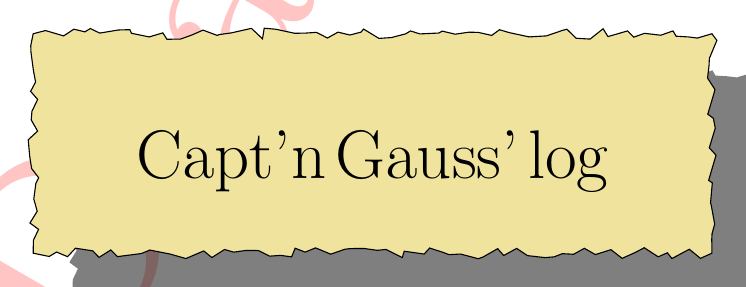
\begin{tikzpicture}[pencildraw/.style={ %
    decorate,
    decoration={random steps,segment length=4pt,amplitude=2pt}
    } %
]
\node[
preaction={fill=black,opacity=.5,transform canvas={xshift=.5cm,yshift=-.5cm}},
pencildraw,draw,fill=paper,text width=3in,inner sep=.5cm] 
{\begin{center}\Huge Capt'n Gauss' log \end{center}\vspace{.7cm} {\huge\context}};
\end{tikzpicture}}

\end{tabular*}

\vfill

\includegraphics[width=3in]{logoPirate.png}\hfill \includegraphics[width=2in]{bammLogo.png}


}


\begin{document}



\begin{context}
  Mathys! I need yer help to find me secret port. 


  \vspace{1cm}

  
  Prove you're a old seadog like me, help me navigate me ship!


\end{context}



\begin{directions}
  \begin{itemize}
  \item Start at the ``X''.
  \item Use the compass rose to find the direction.
  \item Use the ruler to plot your path.
  \end{itemize}
  
\end{directions}



\begin{example}%%https://www.nicepng.com/downpng/u2r5w7a9y3q8q8u2_pirates-of-the-caribbean-ship-png-clipart-jack/
  Our ship travels 2 days East, 1 day South, 3 days North East. Where are we?
\begin{center}
  \begin{tikzpicture}
    \pic[scale=.5] at (0,2in) {compass};
    \node[left] at (0,0) {\scalebox{2}{X}};
    
    \draw[step=2.0in,black,ultra thick,dashed] (0,0) -- (2in,0in) -- (2in,-1in) -- (5in,2in);
    \node[above right] at (5in,2in) {\scalebox{-1}[1]{\includegraphics[width=1in]{pirateship.png}}};
\end{tikzpicture}
\end{center}
\end{example}



\begin{mathConnections}
    https://bartsnapp.github.io/Math-Outreach-Exhibits/deadReckoning/
\end{mathConnections}
\end{document}
